The "Back Burner Brew" is built with the sole purpose of brewing large batch of beer in the home environment. This product provides home brewers with a low-cost electric home brewing system that allow them to have precise control over the brewing process. The brewing process can be automated with the help of micro-controllers like the ESP32 which is then hosted to a local website or an app interface.

\subsection{Purpose and Use}
ESP32 is a micro-controller that can receive data such as current temperature of the water or mash from the heat sensors located inside the kettles which can be converted to either analog or digital input. The heating coil can be control using the input from the user as per their desired either to increase or to decrease the temperature. The electric pump can also be controlled by the user through micro-controller to regulate the flow of the water in the kettles. The user will be able to communicate with the brewing system through a web interface or app interface.

\subsection{Intended Audience}
The foremost intended audiences for this product would be home brewers or person interested in brewing beer only. Provided that the user manual would be present in the product, any person who wants to brew beer in his local environment can easily use this product. This product is made focusing on how effortless can the brewing process gets simply with the use of micro-controller.

\begin{figure}[H]
	\centering
	\graphicspath{.\images}
	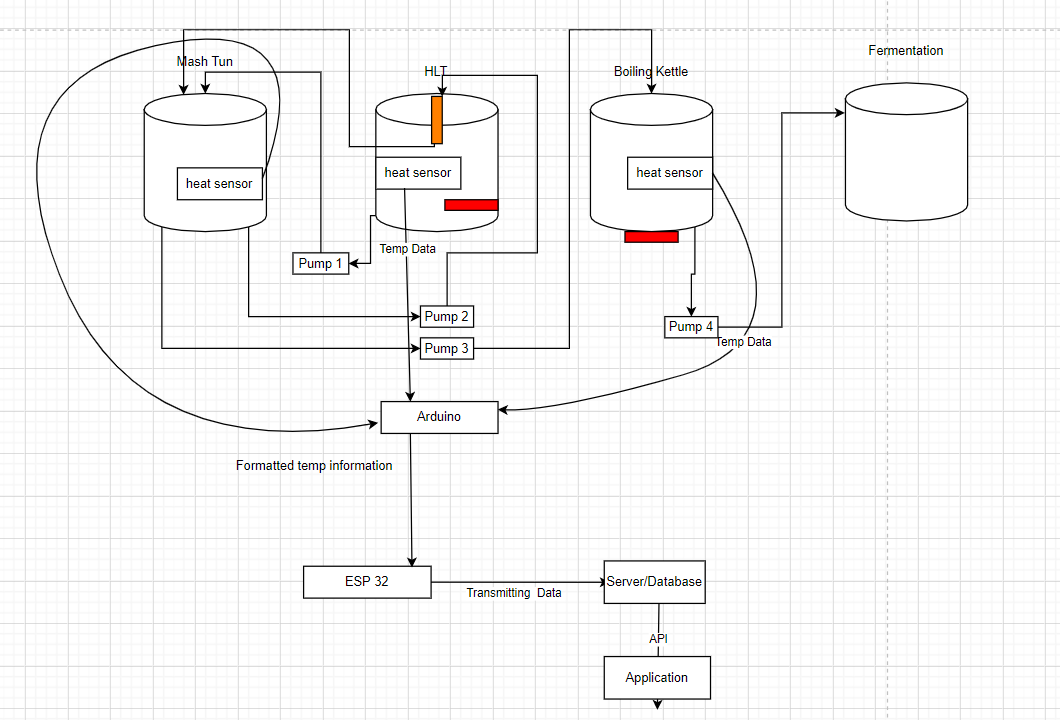
\includegraphics[scale=0.5]{images/sys_overview.PNG}
	\caption{Product Concept}
\end{figure}